\documentclass[10pt]{article}
\usepackage[utf8]{inputenc}

\usepackage{amsfonts}
\usepackage{amsmath}
\usepackage[T2A]{fontenc}
\usepackage[english,russian]{babel}

%\usepackage[dvips]{graphicx}
%\DeclareGraphicsExtensions{.pdf,.png,.jpg}
%\usepackage[dvips]{color} english,

\usepackage{graphicx}
\graphicspath{{Pic/}}
\DeclareGraphicsExtensions{.pdf,.png,.jpg}

\newcommand{\specialcell}[2][c]{%
  \begin{tabular}[#1]{@{}c@{}}#2\end{tabular}}

\usepackage{amsmath}

\textwidth=14 cm
\textheight=20 cm

\begin{document}

\large \noindent  УДК 51-72, 51-74, 519.688

\bigskip

 В. Г. Дружинин, В. А. Морозов
 
\begin{center}
\bf ТРЕХМЕРНАЯ МОДЕЛЬ, ОПИСЫВАЮЩАЯ ОТКЛОНЕНИЯ АСИММЕТРИЧНОЙ ИГЛЫ ПРИ ДВИЖЕНИИ В МЯГКИХ ТКАНЯХ
\end{center}

\bigskip
\textbf{1. Введение}

\bigskip
В наши дни роботы все больше заменяют ручной труд человека. Машины уже могут выполнять не только монотонные производственные действия, но и заменять человека в более сложных операциях. К примеру можно отнести выполнение медицинских операций, как мало инвазивных, так и полноценных операций.
В настоящей статье рассматриваеться проведение операций брахитерапии рака предстательной железы (РПЖ). На сегодняшний день в ЦНИИ РТК разработан макет роботизированной системы «ОнкоРОБОТ») для проведения таких операций ~\cite{one, two}. 
Данная процедура проводится посредством внедрения микроисточников радиоизлучения в предстательную железу максимально близко к опухоли. Основная сложность заключается в подведения кончика иглы к целевой точке (опухоли) при проведении операции.
Преимущества использования роботов по сравнению с традиционными методами заключаются в том, что роботизированный манипулятор способен обеспечить более высокую точность наведения инструмента чем человек, а также контролировать силовое воздействие, что позволяет рассчитывать не только на повышение качества освоенных в настоящее время операций, но и на создание базиса для разработки принципиально новых хирургических технологий. 
Другим важным преимуществом является отсутствие прямого контакта врача с радиоактивными источниками, что позволит обезопасить медицинский персонал от сопутствующего радиационного облучения.
Из-за своих геометрических особенностей и прилагаемых нагрузок в процессе выполнения операции игла деформируется, что приводит к отклонению иглы от прямолинейного движения. 
В работе ~\cite{three} приведен разбор этапов разработки модели приведен анализ существующих методов и подходов, представлена двухмерная модель, описывающая отклонение иглы при движении в тканях человека. 
В данной работе будет решена задача позиционирования иглы в системе координат Оxyz, а также рассмотрены способы повышения точности модели. 
Управление движением иглы осуществляется путем ее поворота иглы вокруг своей оси. При этом кончик иглы поворачивается, а вместе с ним и плоскость изгиба дуги, 
и тем самым изменяется направление дальнейшего движения.
Разработанную модель можно использовать для построения “MPC-регуляторов” – систем, работающих на основе предсказывающих моделей (Model predictive control).
В статье ~\cite{four} показан ход разработки такой системы, только подход для проектирования модели использовался иной. В ~\cite{four} авторы использовали уравнение Лагранжа для определения положения кончика иглы. Также условия эксперимента и сама игла значительно отличались от тех, которые будут рассмотрены в данной работе.

\bigskip
\textbf{2. Модель}

\bigskip
\textbf{2.1 Двумерная модель}

\bigskip
Сначала рассмотрим двумерную модель.
Необходимо разработать такую модель, которая позволяет прогнозировать и корректировать движение иглы в тканях человека.  В данной работе в качестве моделируемого объекта представляется стальная медицинская инъекционная игла длиной 100 мм, диаметром 1 мм с различными углами кончика (рисунок \ref{n1}).
Для построения модели рассмотрим  уравнение равновесия сил при движении иглы ~\cite{Model}: 

\begin{equation} \label{eq1}
\Vec{F}_{needle} = \Vec{F_{t}} + \Vec{F_{f}} + \Vec{w}(x),
\end{equation}
где $\Vec{F_{t}}$ --- сила, действующая на кончик иглы, $\Vec{F_{f}}$ --- сила трения, $\Vec{w}(x)$ --- распределенная нагрузка, $\Vec{F}_{needle}$ --- сила с которой внедряется игла.

\begin{figure}[h]
\center{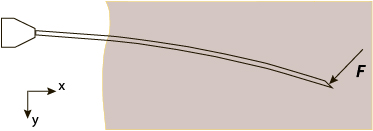
\includegraphics[scale=0.8]{n1.jpg}}
\caption{Форма используемой иглы, F – сила реакции среды}
\label{n1}
\end{figure}

В данной работе будет рассмотрена  задача в следующей постановке:

\begin{equation} \label{eq2}
\Vec{F}_{needle} = \Vec{F_{t}}.
\end{equation}
Для решения поставленной задачи отклонение кончика и угол отклонения будем рассчитывать по формулам ~\cite{Model}:

\begin{equation} \label{eq3}
y_{n} = Fl(t)^3 / 2EJ_{x},
\end{equation}

\begin{equation} \label{eq4}
\theta = Fl(t)^2 / 3EJ_{x},
\end{equation}
где $n$ --- текущая итерация моделирования, $y_{n}$ --- отклонение кончика иглы, на текущем шаге времени,
$F$ --- сила действующая на кончик иглы, $J_{x}$ --- осевой момент инерции, 
$l(t)$ --- длина иглы, находящаяся в тканях человека, $t$ --- время, $E$ --- модуль Юнга, $\theta$ --- угол отклонения.

Для моделирования внешней силы F при перемещении иглы в тканях человека будет использована сила лобового сопротивления:
c\begin{equation} \label{eq5}
F = C \rho v^2 S /2, 
\end{equation}
где $C$ --- коэффициент сопротивления, $\rho$ --- плотность, $v$ --- скорость перемещения иглы, $S$ --- характерная площадь тела, $S = V^{(2/3)}$, где $V$- объем тела.

Для расчета смещения иглы по выражениям \eqref{eq3} и \eqref{eq4} необходимо учитывать проекцию силы F на ось иглы.
В данной постановке задачи по предложенным выражениям \eqref{eq3}, \eqref{eq4}, \eqref{eq5}, будем рассчитывать отклонение итерационно, суммируя его с предыдущими шагами. Тем самым будет сохраняться отклонение на каждом шаге моделирования:

\begin{equation} \label{eq6}
y_{all} = \sum\limits_{1}^{n-1} y_{n},
\end{equation}
где $n$ --- текущая итерация моделирования, $y_{all}$ --- суммарное отклонение иглы при ее движении в тканях человека, $y_{n}$ --- отклонение кончика иглы, на текущем шаге времени.


\bigskip
\textbf{2.2 Трехмерная модель}

Для трехмерной модели используем систему координат, представленную на рисунке \ref{n2}. В данном случае углом поворота будет считаться величина, на которую повернётся плоскость среза иглы.

\begin{figure}[h]
\center{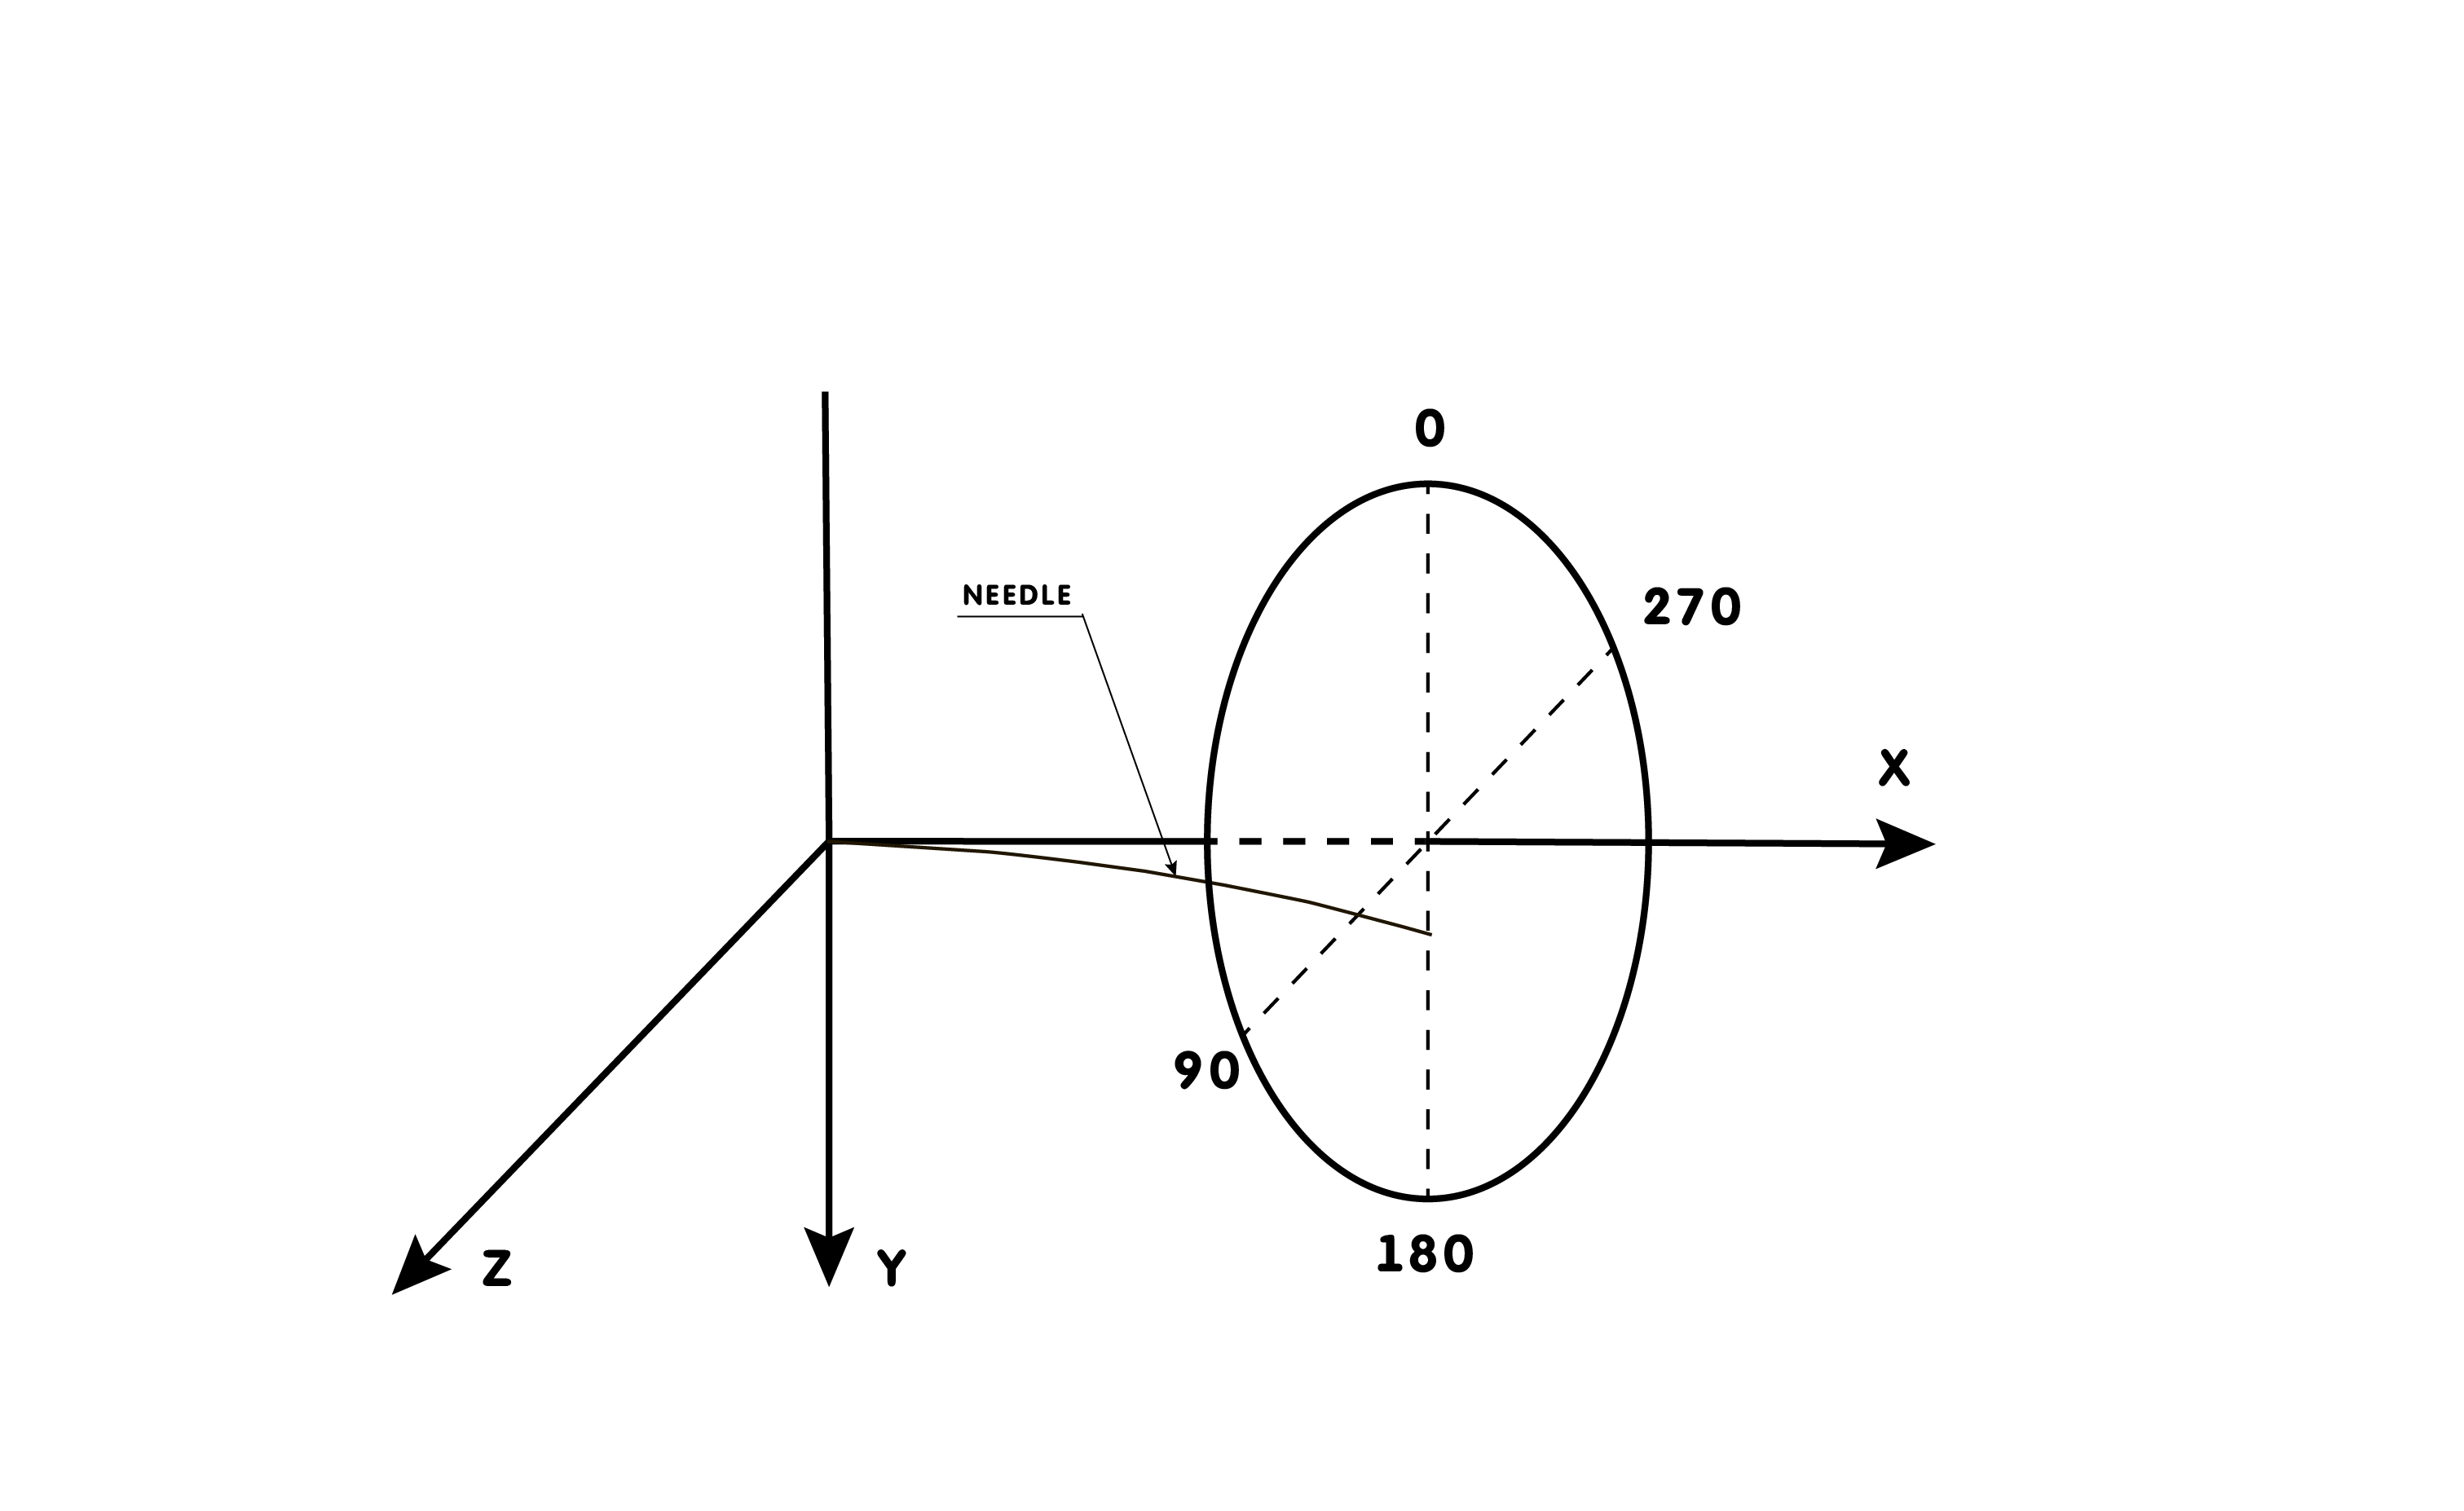
\includegraphics[scale=0.5]{n2.jpg}}
\caption{Рассматриваемая система координат}
\label{n2}
\end{figure}

Для расчета координат положения кончика иглы воспользуемся следующими выражениями:

\begin{equation} \label{eq7}
z_{n} = 
 \begin{cases}
   y_{n} sin(\gamma) &{ 0 \leq \gamma \leq \pi/2 }\\
   y_{n} sin(\pi - \gamma) &{ \pi/2 \leq \gamma \leq \pi }\\
  - y_{n} sin( \gamma - \pi) &{ \pi \leq \gamma \leq 3\pi/2 }\\
   - y_{n} sin(2\pi -  \gamma) &{ 3\pi/2 \leq \gamma \leq 2\pi }\\
 \end{cases}
\end{equation}

\begin{equation} \label{eq8}
z_{all} = \sum\limits_{1}^{n} z_{n},
\end{equation}

\begin{equation} \label{eq9}
y_{k} = 
 \begin{cases}
   y_{n} cos(\gamma) &{ 0 \leq \gamma \leq \pi/2 }\\
   - y_{n} cos(\pi - \gamma) &{ \pi/2 \leq \gamma \leq \pi }\\
  - y_{n} cos( \gamma - \pi) &{ \pi \leq \gamma \leq 3\pi/2 }\\
    y_{n} cos(2\pi -  \gamma) &{ 3\pi/2 \leq \gamma \leq 2\pi }\\
 \end{cases}
\end{equation}

\begin{equation} \label{eq10}
y_{all} = \sum\limits_{1}^{k} y_{k},
\end{equation}
где $\gamma$ --- угол, на который повернулась игла за время моделирования, $z_{all} $ --- компонента отклонения по оси Oz, $y_{all}$ --- компонента отклонения по оси Oy, $y_{n}$ --- отклонение за 1 такт выполнения модели.

Для расчета отклонения от оси Ox воспользуемся следующими выражением:
\begin{equation} \label{eq11}
d_{all} = \sqrt{y_{all}^2  +  z_{all} ^2},
\end{equation}
где $d$ --- общее отклонение кончика игла от оси Ox.

Таким образом, на каждом шаге моделирования будет анализироваться угол, на который повернулась игла. Затем будет вычисляться отклонение на данном шаге и переводиться в координаты. А из данных значений координат y и z вычисляется общее отклонение от оси Ox.
Далее рассмотрены результаты моделирования и приведено сравнение с экспериментальными данными.

\bigskip
\textbf{2.3 Расчет коэффициентов сопротивления}

Решаемая задача является многопараметрической и зависит от нескольких переменных, а именно от поступательной и вращательной скоростей движения иглы в тканях. Необходимо найти такое решение, чтобы различие между экспериментальными и расчетными данными было минимальным. 
Результаты моделирования по двухмерной модели с постоянным коэффициентом C, взятым из справочника, показали достаточно большие погрешности. 

Исходя из этого, данный коэффициент будем представлять в виде некоторой функциональной зависимости от скорости перемещения иглы, построенной на основе экспериментальных данных.  Данный подход позволил  обеспечить минимальные погрешности при моделировании.

Далее рассмотрим коэффициенты для различных вращательных скоростей 0, 3, 4, 5 рад/сек.  

Для вращательной скорости равной 0 рад/сек:
\begin{multline} \label{eq12}
C= 2.2293\cdot10^{11} v^6 - 2.5517\cdot10^{10} v^5+1.788\cdot10^9 v^4 - \\ -2.8053\cdot10^7 v^3 +3.6420\cdot10^5 v^2-2.4583\cdot10^3 v+7.4299.
\end{multline}
Для вращательной скорости равной 3 рад/сек:
\begin{multline} \label{eq13}
C= -6.1243\cdot10^{18} v^9 + 1.0095\cdot10^{18}v^8 -  7.2393\cdot10^{16} v^7 +\\+ 2.9601\cdot10^{15} v^6 - 7.5961\cdot10^{13} v^5 + 1.2673\cdot10^{12} v^4 - \\-1.3740\cdot10^{10} v^3 + 9.3490\cdot10^7 v^2 - 3.6459\cdot10^5 v+ 634.2858.
\end{multline}
Для вращательной скорости равной 4 рад/сек:
\begin{multline} \label{eq14}
C= -5.5744\cdot10^{18} v^9 + 9.29\cdot10^{17}v^8 -  6.7439\cdot10^{16} v^7 +\\+ 2.7959\cdot10^{13} v^6 - 7.2889\cdot10^{13} v^5 + 1.2385\cdot10^{12} v^4 - \\-1.3720\cdot10^{10} v^3 + 9.5768\cdot10^7 v^2 - 3.3892\cdot10^5 v+ 693.0468.
\end{multline}
Для вращательной скорости равной 5 рад/сек:
\begin{multline} \label{eq15}
C= -1.5127\cdot10^{19} v^9 + 2.4827\cdot10^{18}v^8 -  1.7730\cdot10^{17} v^7 +\\+ 7.2242\cdot10^{15} v^6 - 1.8491\cdot10^{14} v^5 + 3.082\cdot10^{12} v^4 - \\-3.3464\cdot10^{10} v^3 + 2.2881\cdot10^7 v^2 - 9.0014\cdot10^5 v+ 1.5829\cdot10^3.
\end{multline}

В  таблице \ref{table1} представлены результаты расчетов коэффициентов для различных поступательных и вращательных скоростей по выражениям \eqref{eq12}, \eqref{eq13}, \eqref{eq14}, \eqref{eq15}.

\begin{table}[h]
\caption{Коэффициенты лобового сопротивления}
\label{table1}
\begin{center}
\begin{tabular}{ | c | c | c | c | c | }
\hline
 & \multicolumn{4}{c|}{Коэффициенты С}   \\ 
 \cline{2-5}
 \raisebox{1.5ex}[0cm][0cm] {\specialcell{Линейная \\ скорость,  мм/с}} & 0 рад/с & 2 рад/с & 4 рад/с & 5 рад/с \\ \hline
3   &  2,664938602	& 97,13340693	& 114,2592189	& 247,5463059 \\ \hline
6	& 1,07169768	& 15,73135406	& 19,05791457	& 38,10638623 \\ \hline
9	& 0,700671524	& 6,365846027	& 7,064884636	& 13,06272217 \\ \hline
12	& 0,659327251	& 3,23079564	& 3,700963655	& 6,112620422 \\ \hline
15	& 0,660593963	& 1,842929895	& 2,20407716	& 3,438567258 \\ \hline
18	& 0,688335976	& 1,204554851	& 1,455901558	& 2,214430941 \\ \hline
21	& 0,779838013	& 0,795031504	& 0,941747061	& 1,480803942 \\ \hline
24	& 0,925302352	& 0,559047066	& 0,662773618	& 1,06863687  \\ \hline
27	& 1,084357932	& 0,403247032	& 0,498425997	& 0,792121034 \\ \hline
30	& 1,319581413	& 0,312718332	& 0,380221049	& 0,626483873 \\ \hline
\end{tabular}
\end{center}
\end{table}

\bigskip
\textbf{3. Результаты моделирования}
 
Моделирование проводилось для различных начальных значений. При моделировании использовались следующие поступательные скорости: 3, 6, 9, 12, 15, 18, 21, 24, 27, 30 мм/с. Рассматривались следующие вращательные скорости: 0, 3, 4, 5 рад/c.  Для различных вращательных скоростей использовались соотвествующие полиномы для расчета коэффициента лобового сопротивления. 
В таблице \ref{table2}  приведены результаты моделирования.

\begin{table}[h]
\caption{Отклонение иглы от прямолинейного движения}
\label{table2}
\begin{center}
\begin{tabular}{ | c | c | c | c | c | }
\hline
 & \multicolumn{4}{c|}{Отклонение, мм}   \\ 
 \cline{2-5}
 \raisebox{1.5ex}[0cm][0cm] {\specialcell{Линейная \\ скорость,  мм/с}} & 0 рад/с & 2 рад/с & 4 рад/с & 5 рад/с \\ \hline
3	& 0,10	& 0,17	& 0,15	& 0,26 \\ \hline
6	& 0,16	& 0,22	& 0,20	& 0,32 \\ \hline
9	& 0,24	& 0,30	& 0,25	& 0,37 \\ \hline
12	& 0,40	& 0,36	& 0,31	& 0,41 \\ \hline
15	& 0,62	& 0,40	& 0,36	& 0,45 \\ \hline
18	& 0,93	& 0,45	& 0,41	& 0,50 \\ \hline
21	& 1,43	& 0,47	& 0,42	& 0,53 \\ \hline
24	& 2,22	& 0,49	& 0,44	& 0,57 \\ \hline
27	& 3,29	& 0,50	& 0,47	& 0,60 \\ \hline
30	& 4,94	& 0,53	& 0,49	& 0,65 \\ \hline
\end{tabular}
\end{center}
\end{table}

Погрешности при моделировании с использованием подобранных коэффициентов лобового сопротивления не превышают 0.01 мм.

 
\bigskip
\textbf{4. Заключение}

В ходе выполнения данной работы были разработаны 2-х мерная и 3-х мерная модели, описывающие отклонение медицинской инъекционной иглы от прямолинейного движения при движениях в тканях человека.
С целью наибольшего приближению расчетных данных к экспериментальным, осуществлен подбор коэффициентов  лобового сопротивления С при проведении моделирования.
Проведено моделирование при различных начальных условиях.
Результаты моделирования с использованием подобранных коэффициентов С показывают, что данная модель может использоваться в робототехнических системах для прогнозирования движения или  использоваться для проектирования "МРС-регуляторов". Данная модель так же может быть использована для проведения виртуальных операций с инъекциями.


 
\bigskip
\begin{thebibliography}{99}
\small

\bibitem{one}{Н.А. Грязнов, Г.С. Киреева, В.В. Харламов, К.Ю. Сенчик, Д.В. Новицкий, С.А. Никитин.}{\; Управление роботом для брахитерапии на основе информации ультразвукового датчика // Робототехника и техническая кибернетика. 1(10). 2016. С 67-71.}
\bibitem{two}{Н.А. Грязнов, Г.С. Киреева, В.В. Харламов, К.Ю. Сенчик, Д.В. Новицкий, С.А. Никитин.}{\; Перспективы использования оригинальной роботизированной системы для брахитерапии рака предстательной железы // Вестник хирургии им. И.И. Грекова. Том 176, выпуск 1. 2017. С 107-111.}
\bibitem{three}{Elliott D. M. }{\; Automated implantation system for radioisotope seeds // U.S. patent 6869390 B2 (22 March 2005).}
\bibitem{four}{Fichtinger G.}{\; System for robotically assisted prostate biopsy and therapy with intraoperative CT guidance // Acad. Radiol. – 2002. – Vol. 9. – P. 60–74.}
\bibitem{Model}{В.Г. Дружинин, В.А. Морозов, С.А. Никитин, В.В. Харламов.}{\; Модель Отклонения медицинской иглы при движении в тканях человека //Российский журнал биомеханики выпуск 4 2018 С 459-472.}

\end{thebibliography}

\end{document}

